\chapter{Conclusioni e sviluppi futuri}
\section{Conclusioni}
In questo lavoro di tesi è stata presentata QRChain, un modello di blockchain basata su Proof-of-Stake, con lo scopo di introdurre problemi e soluzioni delle attuali blockchain in vista del sempre più rapido sviluppo dei computer quantistici. Come primo passo sono state analizzate le vulnerabilità note delle blockchain odierne. La prima vulnerabilità riguarda gli attacchi effettuati tramite l'algoritmo di ricerca di Grover e l'algoritmo di fattorizzazione di Shor. Successivamente, sono state fatte le considerazioni sulla progettazione del sistema blockchain. La soluzione adottata si basa sulla sostituzione dell'attuale schema di firma digitale sostituendo il vecchio, non quantum-safe, con uno sicuro. La scelta dello schema di firma è ricaduta sullo SPHINCS che risulta essere quantum-safe oltre che adatto al nostro caso.

\section{Sviluppi futuri}
% \subsection{Ethereum 2.0}
% Tra gli sviluppi futuri si propone un aggiornamento di Ethereum sostituendo l'attuale algoritmo di consenso utilizzato, la Proof-of-Work, con il più sicuro e sostenibile Proof-of-Stake. Così facendo si crea una base su cui poi andare ad applicare la nostra implementazione, QRChain, per rendere Ethereum sicuro agli attacchi quantistici.

% Il passaggio verso PoS permetterà di concretizzare meglio quella che è stata la visione originaria che ha portato alla realizzazione di Ethereum, passando ad una rete più scalabile, più sicura e più sostenibile. E in particolare il tema della sostenibilità, poiché con il passaggio a PoS Ethereum promette di abbattere del 99,95\% il consumo energetico necessario per il funzionamento della rete, come possiamo vedere nella Figura \ref{fig:pos_energy}.

% \begin{figure}[h]
%   \centering
%   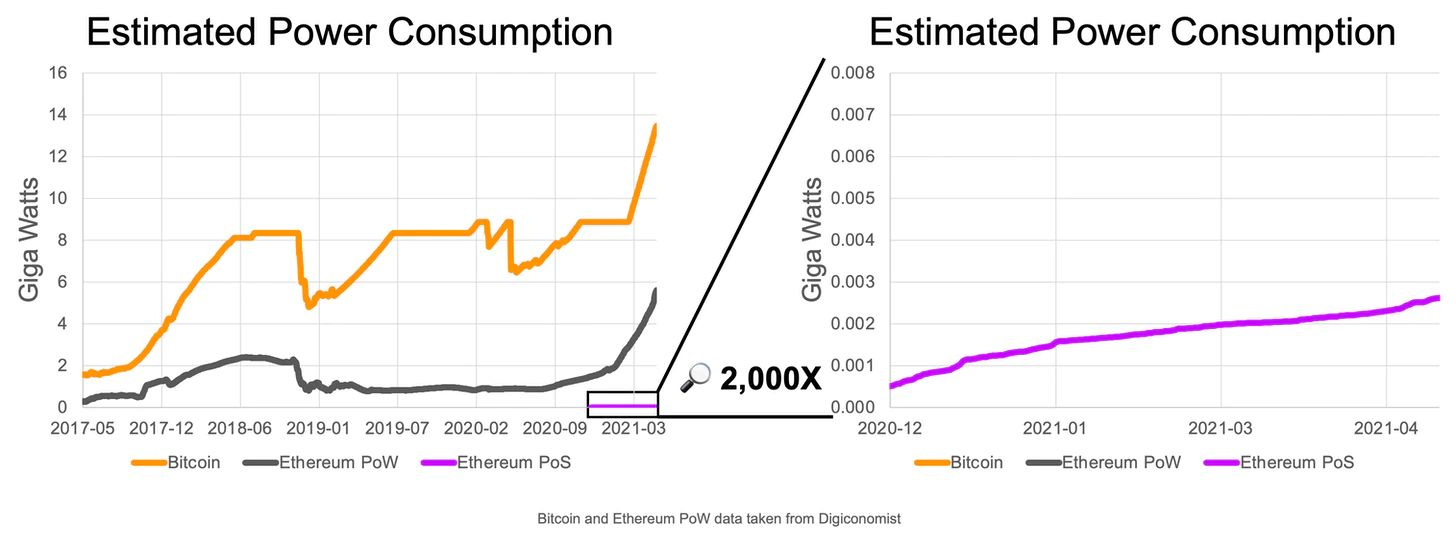
\includegraphics[width=0.7\textwidth]{pos_energy.jpeg}
%   \caption{Consumo energetico da parte di Bitcoin ed Ethereum}
%   \label{fig:pos_energy}
% \end{figure}

% Questa migrazione da PoW a PoS può avvenire tramite un \textit{merge} e non tramite un hard fork del sistema. Infatti, con il termine merge, indichiamo la fusione del client di esecuzione della mainnet Ethereum con il client di consenso \textit{Beacon Chain Proof-of Stake}. Nonostante il termine Eth 2.0 o Ethereum 2.0, Il merge è in realtà un aggiornamento della rete e non la creazione di un nuovo token o di una nuova rete, come potrebbe far pensare il termine "Eth2". Dopo questa fusione, i nodi Ethereum comprenderanno sia un client di esecuzione (Eth1) che un client di consenso (Eth2); entrambi sono necessari per far funzionare un nodo Ethereum completo dopo la fusione.

% \begin{figure}[h]
%   \centering
%   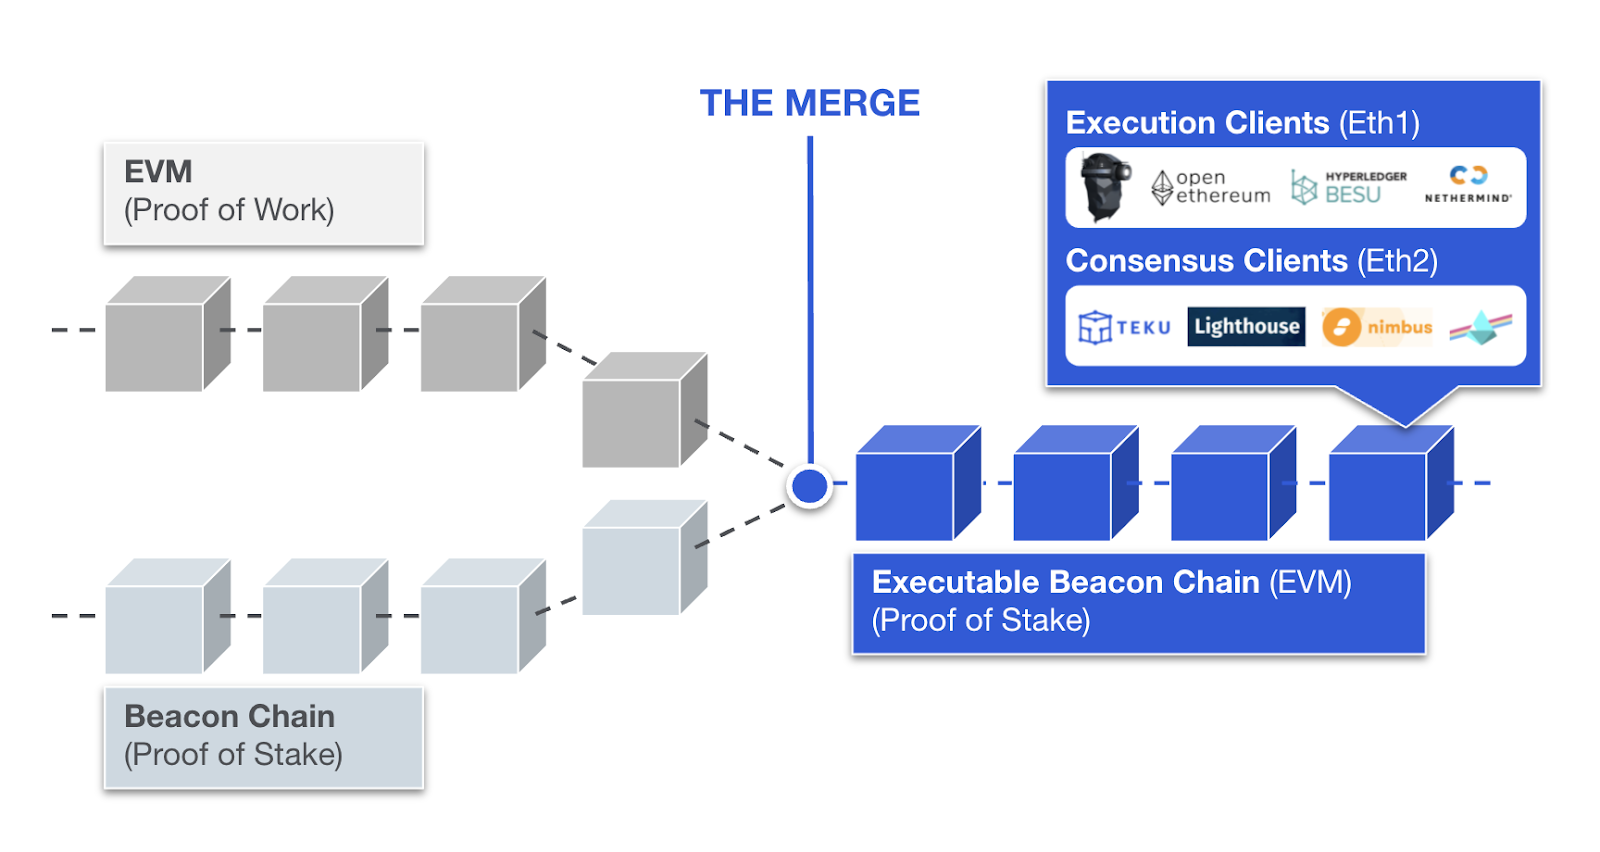
\includegraphics[width=0.7\textwidth]{the_merge.png}
%   \caption{Migrazione da Ethereum a Ethereum 2.0}
%   \label{fig:the_merge}
% \end{figure}

\subsection{SPHINCS+}
Infine, un ulteriore sviluppo futuro proposto è la sostituzione dello SPHINCS con il più recente SPHINCS+.

SPHINCS+ è uno schema di firma stateless basato su hash, presentato al progetto di crittografia post-quantistica del NIST \cite{Bernstein2017SPHINCSS}. Il progetto è un'evoluzione dello schema di firma SPHINCS, presentato a EUROCRYPT 2015. Incorpora diversi miglioramenti, mirati in particolare a ridurre la dimensione della firma e velocizzare lo schema. Lo SPHINCS+, in termini di progettazione, è analogo allo SPHINCS, ma modificando alcuni aspetti interni. Riassumiamo di seguito i principali cambiamenti dello SPHINCS+:
\begin{description}
  \item[Protezione dagli attacchi multitarget] Ad ogni chiamata viene utilizzata una hash function diversa con una chiave diversa applicando differenti bitmask. Le chiavi e le bitmask sono generati pseudo-randomicamente da un indirizzo specificando il contesto della chiamata, e un seme pubblico.
  \item[Tree-less WOTS+ public key compression] Gli ultimi nodi della catena WOTS+ non vengono compressi usando una singola funzione hash. Come prima, viene chiamata una funzione hash diversa ad ogni invocazione.
  \item[FORS] Lo schema di firma HORST è stato rimpiazzato con il \textit{FORS (Forest Of Random Subset)}. Una coppia di chiavi FORS non consiste di un singolo albero monolitico ma di \(k\) alberi di altezza \(\log t\). Il vantaggio è che ora si possono utilizzare parametri molto più piccoli e quindi, alla fine, guadagnare in dimensione e velocità della firma.
  \item[Selezione dell'indice verificabile] In SPHINCS la coppia di chiavi HORST utilizzata per firmare il messaggio veniva selezionata generando un indice in modo pseudorandom. Poiché si trattava di un valore di seme segreto, un verificatore non era in grado di controllare se l'indice fosse stato effettivamente generato in quel modo.  Ciò comportava lo svantaggio che un avversario che avesse preso di mira HORST avrebbe potuto sferrare un attacco multi-target, utilizzando un calcolo dell'hash per colpire tutte le istanze HORST contemporaneamente. Questo non è più possibile. SPHINCS+ calcola l'indice insieme al message digest come \(( md \| idx ) = H ( R, PK, M )\) dove PK è la chiave pubblica di SPHINCS+ e R è un valore (pseudo-)generato casualmente che diventa parte della firma. In questo modo, ogni messaggio che un avversario tenta di trasmettere diventa direttamente collegato a un'istanza FORS ed è inutilizzabile per qualsiasi altra istanza. Inoltre, questo ci permette di omettere l'indice nella firma SPHINCS+.
\end{description}